\documentclass[10pt]{article}

\usepackage[landscape,margin=0.55in]{geometry}
\usepackage[T1]{fontenc}
\usepackage[utf8]{inputenc}
\usepackage{lmodern}
\usepackage{xcolor}
\usepackage{graphicx}
\usepackage{tikz}
\usetikzlibrary{arrows.meta,positioning,shapes.geometric,fit}

\definecolor{phaseblue}{HTML}{C2E5FF}
\definecolor{phasebluestroke}{HTML}{3DADFF}
\definecolor{successgreen}{HTML}{CDF4D3}
\definecolor{successstroke}{HTML}{66D575}
\definecolor{failred}{HTML}{FFCDC2}
\definecolor{failstroke}{HTML}{FF7556}
\definecolor{warnorange}{HTML}{FFE0C2}
\definecolor{warnstroke}{HTML}{FF9E42}
\definecolor{mutedgray}{HTML}{F2F2F2}
\definecolor{mutedstroke}{HTML}{B3B3B3}

\tikzset{
  flow/.style={
    rectangle,
    rounded corners=2pt,
    draw=phasebluestroke,
    fill=phaseblue,
    minimum width=2.55cm,
    minimum height=1.05cm,
    text width=2.35cm,
    align=center,
    font=\small
  },
  decision/.style={
    diamond,
    aspect=2.1,
    draw=warnstroke,
    fill=warnorange,
    minimum width=2.45cm,
    minimum height=1.15cm,
    text width=1.75cm,
    align=center,
    inner sep=1pt,
    font=\small
  },
  failure/.style={
    rectangle,
    rounded corners=2pt,
    draw=failstroke,
    fill=failred,
    minimum width=2.55cm,
    minimum height=0.95cm,
    text width=2.35cm,
    align=center,
    font=\small
  },
  success/.style={
    rectangle,
    rounded corners=5pt,
    draw=successstroke,
    fill=successgreen,
    minimum width=2.65cm,
    minimum height=1.05cm,
    text width=2.45cm,
    align=center,
    font=\small
  },
  artifact/.style={
    rectangle,
    rounded corners=2pt,
    draw=mutedstroke,
    fill=mutedgray,
    minimum width=2.5cm,
    minimum height=0.95cm,
    text width=2.3cm,
    align=center,
    font=\small
  },
  arrow/.style={-{Latex[length=2.5mm]},thick,draw=black!70},
  edgeLabel/.style={font=\scriptsize,fill=white,inner sep=1.5pt},
  method/.style={font=\scriptsize,text=black!70,align=center}
}

\pagestyle{empty}

\begin{document}

\begin{center}
{\Large\bfseries Put Target Object on Target Pad: Execution Flow and Round-3 Outcomes}

\vspace{0.15em}
{\small Source: \texttt{scripts/validation/results/round3\_broad\_sweep\_rollout}, 20 episodes}
\end{center}

\vspace{0.2em}

\resizebox{\textwidth}{!}{%
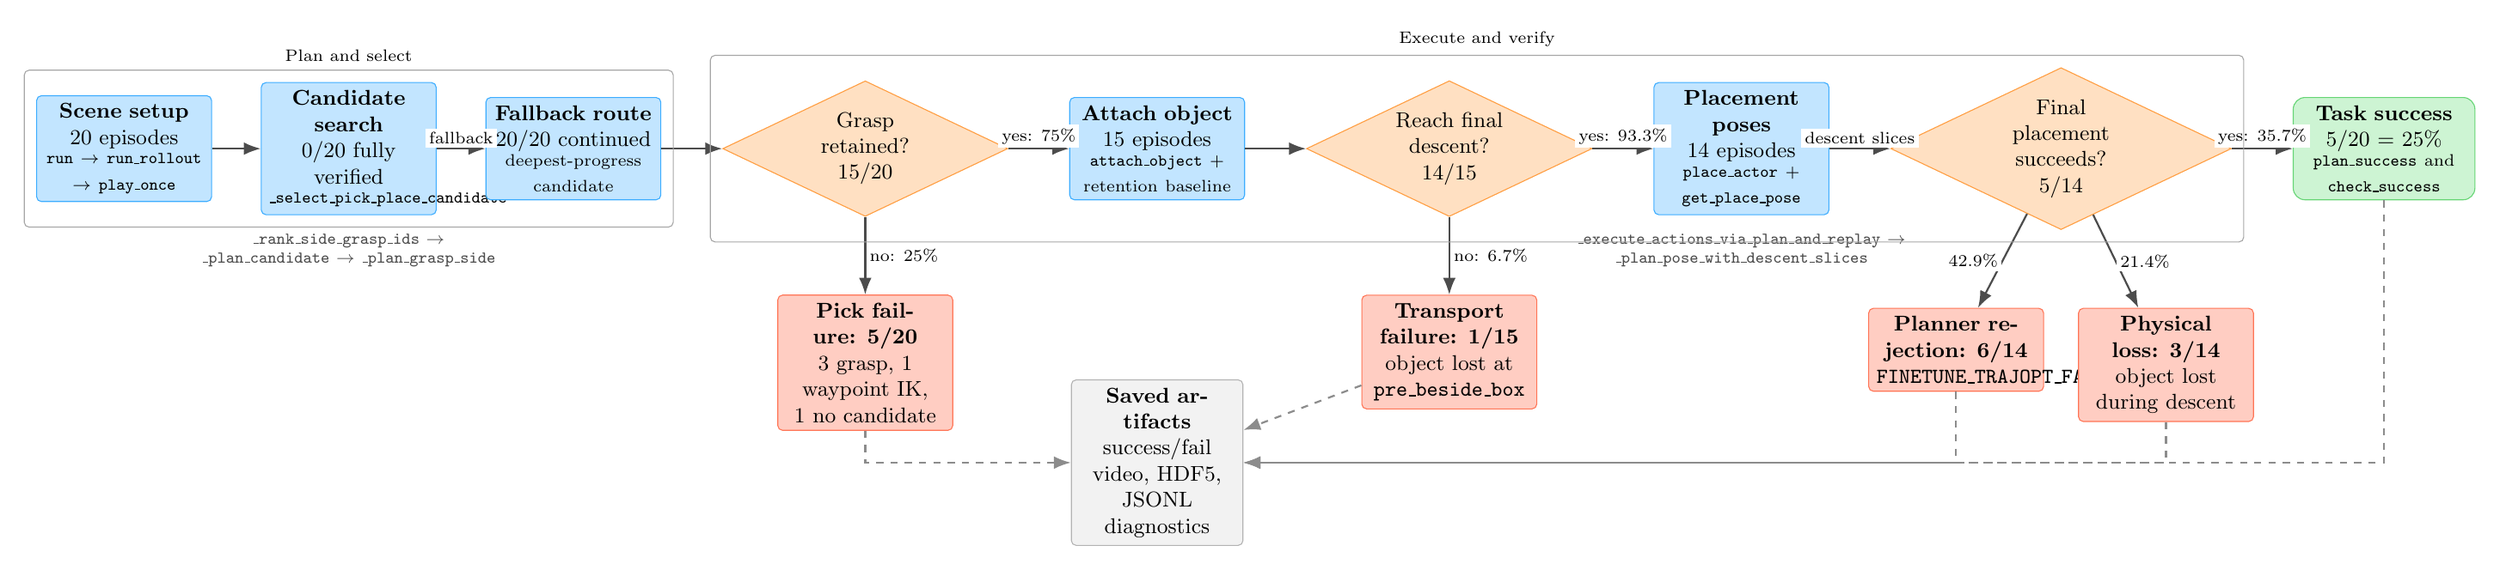
\begin{tikzpicture}[node distance=0.75cm and 0.72cm]
  \node[flow] (setup) {
    \textbf{Scene setup}\\
    20 episodes\\[-1mm]
    {\scriptsize \texttt{run} $\rightarrow$ \texttt{run\_rollout} $\rightarrow$ \texttt{play\_once}}
  };

  \node[flow, right=of setup] (candidate) {
    \textbf{Candidate search}\\
    0/20 fully verified\\[-1mm]
    {\scriptsize \texttt{\_select\_pick\_place\_candidate}}
  };

  \node[flow, right=of candidate] (fallback) {
    \textbf{Fallback route}\\
    20/20 continued\\[-1mm]
    {\scriptsize deepest-progress candidate}
  };

  \node[decision, right=0.9cm of fallback] (grasp) {
    Grasp retained?\\
    15/20
  };

  \node[flow, right=0.9cm of grasp] (attach) {
    \textbf{Attach object}\\
    15 episodes\\[-1mm]
    {\scriptsize \texttt{attach\_object} + retention baseline}
  };

  \node[decision, right=0.9cm of attach] (transport) {
    Reach final descent?\\
    14/15
  };

  \node[flow, right=0.9cm of transport] (place) {
    \textbf{Placement poses}\\
    14 episodes\\[-1mm]
    {\scriptsize \texttt{place\_actor} + \texttt{get\_place\_pose}}
  };

  \node[decision, right=0.9cm of place] (descent) {
    Final placement succeeds?\\
    5/14
  };

  \node[success, right=0.9cm of descent] (taskSuccess) {
    \textbf{Task success}\\
    5/20 = 25\%\\[-1mm]
    {\scriptsize \texttt{plan\_success} and \texttt{check\_success}}
  };

  \node[failure, below=1.15cm of grasp] (pickFail) {
    \textbf{Pick failure: 5/20}\\
    3 grasp, 1 waypoint IK,\\
    1 no candidate
  };

  \node[failure, below=1.15cm of transport] (transportFail) {
    \textbf{Transport failure: 1/15}\\
    object lost at\\
    \texttt{pre\_beside\_box}
  };

  \node[failure, below=1.15cm of descent,xshift=-1.55cm] (descentPlanFail) {
    \textbf{Planner rejection: 6/14}\\
    \texttt{FINETUNE\_TRAJOPT\_FAIL}
  };

  \node[failure, below=1.15cm of descent,xshift=1.55cm] (descentLossFail) {
    \textbf{Physical loss: 3/14}\\
    object lost during descent
  };

  \node[artifact, below=2.65cm of attach] (artifacts) {
    \textbf{Saved artifacts}\\
    success/fail video, HDF5,\\
    JSONL diagnostics
  };

  \draw[arrow] (setup) -- (candidate);
  \draw[arrow] (candidate) -- node[edgeLabel,above]{fallback} (fallback);
  \draw[arrow] (fallback) -- (grasp);
  \draw[arrow] (grasp) -- node[edgeLabel,above]{yes: 75\%} (attach);
  \draw[arrow] (grasp) -- node[edgeLabel,right]{no: 25\%} (pickFail);
  \draw[arrow] (attach) -- (transport);
  \draw[arrow] (transport) -- node[edgeLabel,above]{yes: 93.3\%} (place);
  \draw[arrow] (transport) -- node[edgeLabel,right]{no: 6.7\%} (transportFail);
  \draw[arrow] (place) -- node[edgeLabel,above]{descent slices} (descent);
  \draw[arrow] (descent) -- node[edgeLabel,above]{yes: 35.7\%} (taskSuccess);
  \draw[arrow] (descent) -- node[edgeLabel,left]{42.9\%} (descentPlanFail);
  \draw[arrow] (descent) -- node[edgeLabel,right]{21.4\%} (descentLossFail);

  \draw[arrow,dashed,draw=black!45] (pickFail) |- (artifacts);
  \draw[arrow,dashed,draw=black!45] (transportFail) -- (artifacts);
  \draw[arrow,dashed,draw=black!45] (descentPlanFail) |- (artifacts);
  \draw[arrow,dashed,draw=black!45] (descentLossFail) |- (artifacts);
  \draw[arrow,dashed,draw=black!45] (taskSuccess) |- (artifacts);

  \node[method, below=0.15cm of candidate] {
    \texttt{\_rank\_side\_grasp\_ids} $\rightarrow$\\
    \texttt{\_plan\_candidate} $\rightarrow$ \texttt{\_plan\_grasp\_side}
  };

  \node[method, below=0.15cm of place] {
    \texttt{\_execute\_actions\_via\_plan\_and\_replay} $\rightarrow$\\
    \texttt{\_plan\_pose\_with\_descent\_slices}
  };

  \node[draw=black!35,rounded corners=2pt,fit=(setup)(candidate)(fallback),
        inner sep=5pt,label={[font=\scriptsize]above:Plan and select}] {};
  \node[draw=black!35,rounded corners=2pt,fit=(grasp)(attach)(transport)(place)(descent),
        inner sep=5pt,label={[font=\scriptsize]above:Execute and verify}] {};
\end{tikzpicture}
}

\vfill

\begin{center}
\fcolorbox{warnstroke}{warnorange}{%
  \parbox{0.91\linewidth}{\centering
    \textbf{Main result:} Once grasping succeeds, transport is reliable (14/15, 93.3\%).
    Final placement is the dominant bottleneck: 6 CuRobo near-contact trajectory rejections
    and 3 physical object losses among the 14 episodes that reached descent.
  }
}
\end{center}

\end{document}
